\Chapter{Shuffle}

\section{When Shuffles Don’t Happen}

Spark knows to avoid a shuffle when a previous transformation has already partitioned the data according
to the same partitioner. Consider the following flow:

rdd1 = someRdd.reduceByKey(...)
rdd2 = someOtherRdd.reduceByKey(...)
rdd3 = rdd1.join(rdd2)

Because no partitioner is passed to reduceByKey, the default partitioner will be used, resulting in 
rdd1 and rdd2 both hash-partitioned. These two reduceByKeys will result in two shuffles. If the RDDs have the 
same number of partitions, the join will require no additional shuffling. Because the RDDs are partitioned 
identically, the set of keys in any single partition of rdd1 can only show up in a single partition of rdd2. 
Therefore, the contents of any single output partition of rdd3 will depend only on the contents of a single 
partition in rdd1 and single partition in rdd2, and a third shuffle is not required.

For example, if someRdd has four partitions, someOtherRdd has two partitions, and both the reduceByKeys use 
three partitions, the set of tasks that execute would look like:

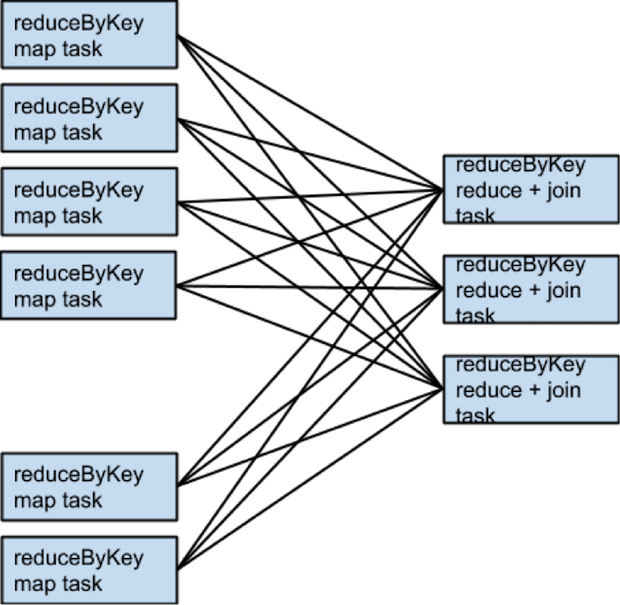
\includegraphics{../../img/spark/spark-tuning-f4.png}

What if rdd1 and rdd2 use different partitioners or use the default (hash) partitioner with different numbers 
partitions?  In that case, only one of the rdds (the one with the fewer number of partitions) will need to be 
reshuffled for the join.

Same transformations, same inputs, different number of partitions:

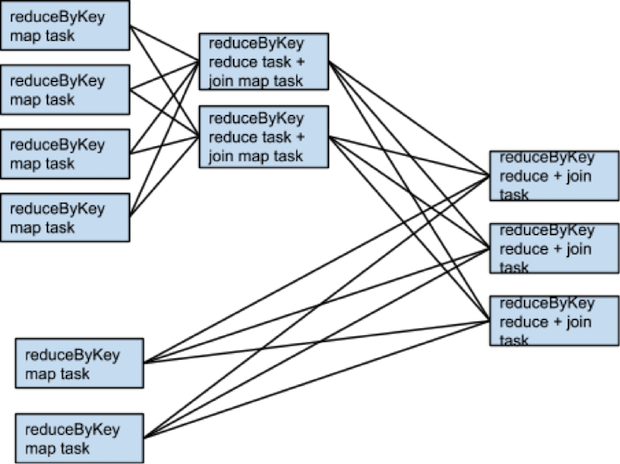
\includegraphics{../../img/spark/spark-tuning-f5.png}

One way to avoid shuffles when joining two datasets is to take advantage of broadcast variables. When one of the 
datasets is small enough to fit in memory in a single executor, it can be loaded into a hash table on the driver and 
then broadcast to every executor. A map transformation can then reference the hash table to do lookups.

\section{When More Shuffles are Better}

There is an occasional exception to the rule of minimizing the number of shuffles. An extra shuffle can be advantageous 
to performance when it increases parallelism. For example, if your data arrives in a \textbf{few large unsplittable files}, 
the partitioning dictated by the InputFormat might place large numbers of records in each partition, while \textbf{not 
generating enough partitions to take advantage of all the available cores}. In this case, invoking \textbf{repartition}
with a high number of partitions (which will trigger a shuffle) after loading the data will allow the operations that come 
after it to leverage more of the cluster’s CPU.

Another instance of this exception can arise when using the reduce or aggregate action to aggregate data into the 
driver. When aggregating over a high number of partitions, the computation can quickly become bottlenecked on a single 
thread in the driver merging all the results together. To loosen the load on the driver, one can first use reduceByKey 
or aggregateByKey to carry out a round of distributed aggregation that divides the dataset into a smaller number of 
partitions. The values within each partition are merged with each other in parallel, before sending their results to 
the driver for a final round of aggregation. Take a look at treeReduce and treeAggregate for examples of how to do that. 
(Note that in 1.2, the most recent version at the time of this writing, these are marked as developer APIs, 
but SPARK-5430 seeks to add stable versions of them in core.)
\textbf{Eg: org.aja.tej.examples.spark.rdd.TreeAgreegate}

This trick is especially useful when the aggregation is already grouped by a key. For example, consider an app that 
wants to count the occurrences of each word in a corpus and pull the results into the driver as a map.  One approach, 
which can be accomplished with the aggregate action, is to compute a local map at each partition and then merge the 
maps at the driver. The alternative approach, which can be accomplished with aggregateByKey, is to perform the count 
in a fully distributed way, and then simply collectAsMap the results to the driver.